 \section{On-policy Control with Approximation}
\subsection{Exercise 10.1}
\subsubsection{Q}
We have not explicitly considered or given pseudocode for any Monte Carlo methods in this chapter. What would they be like? Why is it reasonable not to give pseudocode for them? How would they perform on the Mountain Car task?
\subsubsection{A}
\begin{itemize}
\item Episodes would be rolled-out using an $\epsilon$-soft policy, with states, actions and rewards stored in memory. Then, we loop through each state-action pair visited in the episode updating the weights of our function approximator based on the returns observed thereafter. Control would be performed by following our $\epsilon$-soft policy on the obtained value function. 
\item Pseudocode likely not provided because the algorithm is trivial compared to $n$-step sarsa. 
\item With the monte carlo return being an unbiased estimator of $U_t$, it is possible that monte carlo control could converge on the optimal solution to the mountain car task quicker than $n$-step sarsa.
\end{itemize}

$
\hfill \blacksquare
$

\subsection{Exercise 10.2}
\subsubsection{Q}
Give pseudocode for semi-gradient one-step \textit{Expected}Sarsa for control. 
\subsubsection{A}
$n$-step sarsa pseudocode is:
\begin{figure}[h!]
	\centering
	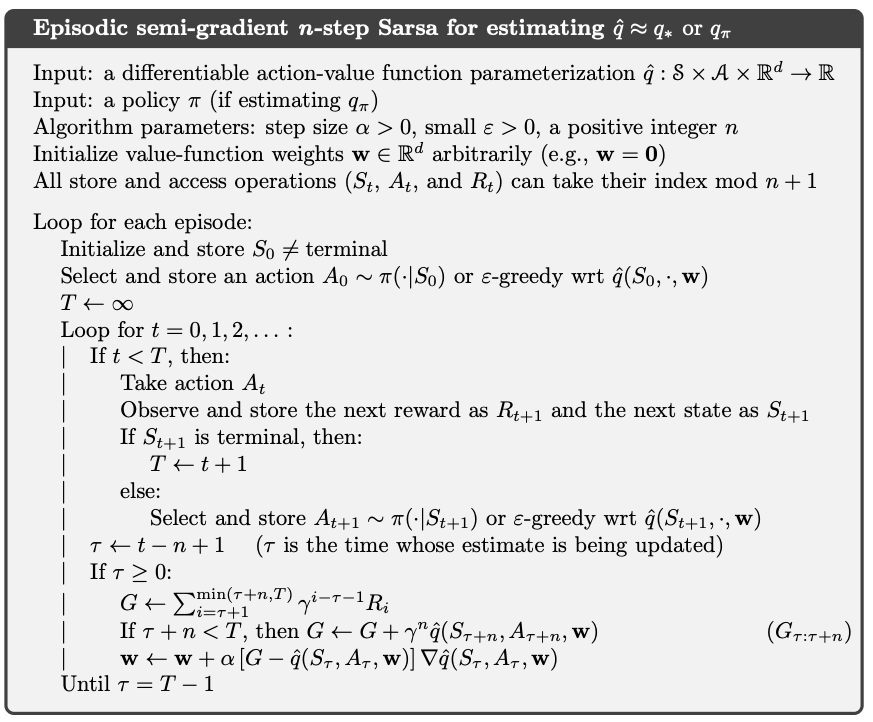
\includegraphics[width=\textwidth]{/chapter10_2}
	\caption{Episodic semi-gradient $n$-step sarsa for estimating $\hat{q} \approx q_*$}
	\label{fig: 10_2}
\end{figure}
The algorithm would be amended to have $n = 1$ and the weight update rule as
\begin{equation}
\textbf{w}_{t+1} \leftarrow \textbf{w}_{t} + \alpha \left[R_{t+1} + \gamma\sum_{a} \pi(a | S_{t+1})\hat{q}(S_t, a, \textbf{w})  - \hat{q}(S_t, A_t, \textbf{w})\right] \nabla \hat{q}(S_t, A_t, \textbf{w})
\end{equation}
$
\hfill \blacksquare
$

\subsection{Exercise 10.3}
\subsubsection{Q}
Why do the results shown in Figure 10.4 have higher standard errors at large $n$ than at small $n$?
\subsubsection{A}
The number of $n$ step permutations grows exponentially in $n$, so the variance of the $n$-step update will grow with $n$.
$
\hfill \blacksquare
$

\subsection{Exercise 10.4}
\subsubsection{Q}
Give pseudocode for a differential version of semi-gradient Q-learning.
\subsubsection{A}
\begin{figure}[h!]
	\centering
	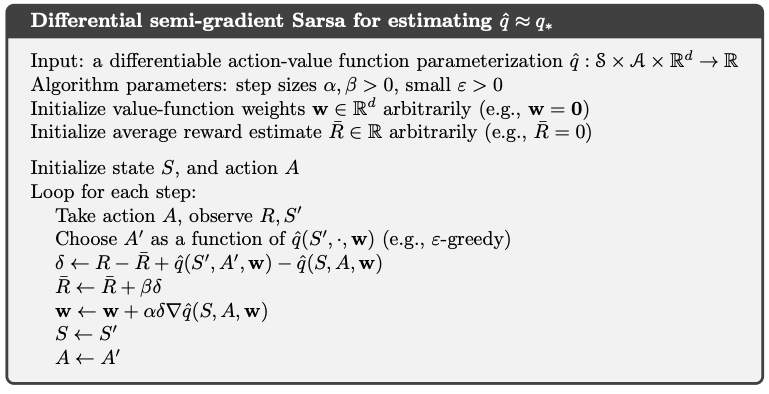
\includegraphics[width=\textwidth]{/chapter10_3}
	\caption{Differential semi-gradient sarsa for estimating $\hat{q} \approx q_*$}
	\label{fig: 10_3}
\end{figure}
Pseudocode for differential semi-gradient sarsa is given in Figure \ref{fig: 10_3}. The algorithm is the same other than the action selection for $A'$ is greedy, not $\epsilon$-greedy.
$
\hfill \blacksquare
$

\subsection{Exercise 10.5}
\subsubsection{Q}
What equations are needed (beyond 10.10) to specify the differential version of TD(0)?
\subsubsection{A}
We need to specify the update to our estimated average return rate $\bar{R}$ and our update to the weights of our function approximator. Which are:
\begin{equation}
\bar{R} \leftarrow \bar{R} + \beta\delta
\end{equation}
and
\begin{equation}
\textbf{w} \leftarrow \textbf{w} + \alpha \delta \nabla \hat{v}(S, \textbf{w})
\end{equation}

\subsection{Exercise 10.6}
\subsubsection{Q}
Suppose there is an MDP that under any policy produces the deterministic sequence of rewards +1, 0, +1, 0, +1, 0,... going on forever. Technically, this violates ergodicity; there is no stationary limiting distribution $\mu_\pi$ and the limit (10.7) does not exist. Nevertheless, the average reward (10.6) is well defined. What is it? Now consider two states in this MDP. From \textbf{A}, the reward sequence is exactly as described above, starting with a +1, whereas, from \textbf{B}, the reward sequence starts with a 0 and then continues with +1, 0, +1, 0,.... We would like to compute the differential values of \textbf{A} and \textbf{B}. Unfortunately, the differential return (10.9) is not well defined when starting from these states as the implicit limit does not exist. To repair this, one could alternatively define the differential value of a state as (see below). Under this definition, what are the differential values of states \textbf{A} and \textbf{B}?
\subsubsection{A}
10.6 is
\begin{align}
r(\pi) &\doteq \lim_{h \rightarrow \infty}\frac{1}{h} \sum_{t=1}^{h} \mathbb{E} \left[R_t | S_0, A_{0:t-1} ~ \pi \right] \\
&= \lim_{h \rightarrow \infty}\frac{1}{h} \sum_{t=1}^{h} 0.5 \\
&= 0.5
\end{align}

and the new expression for the differential value is
\begin{equation}
v_\pi(s) \doteq \lim_{\gamma \rightarrow 1} \lim_{h \rightarrow \infty} \sum_{t=0}^{h} \gamma^t \left(\mathbb{E}_\pi[R_{t+1} | S_0 = s] - r(\pi) \right)
\end{equation}

We can rewrite this as
\begin{align}
v(A; \gamma) &= 0 - \bar{R} + \gamma V(B; \gamma) \\ 
v(B; \gamma) &= 1 - \bar{R} + \gamma V(A; \gamma) \\ 
\end{align}
so 
\begin{align}
v(A; \gamma) &= 0 - \bar{R} + \gamma \left(1 - \bar{R} + \gamma V(A; \gamma)\right) \\
&= \gamma^2 V(A; \gamma) - \bar{R}(1 + \gamma) + \gamma \\
&= \gamma^2 V(A; \gamma) + \frac{1}{2} \gamma - \frac{1}{2} \; \; \text{as} \; \; \bar{R} = 0.5 \\
&= \frac{1}{2} \frac{1 - \gamma}{1 - \gamma^2} \\
&= \frac{1}{2(1+ \gamma)}
\end{align}

So $V(A) = \lim_{\gamma \rightarrow 1} V(A; \gamma) = \frac{1}{4}$ and $V(A; \gamma) = \frac{3}{4}$.

\subsection{Exercise 10.7}
\subsubsection{Q}
Consider a Markov reward process consisting of a ring of three states A, B, and C, with state transitions going deterministically around the ring. A reward of +1 is received upon arrival in A and otherwise the reward is 0. What are the differential values of the three states, using (10.13)?
\subsubsection{A}
We can deduce that $r(\pi) = \frac{1}{3}$. Then we write
\begin{align}
v(A; \gamma) &= 0 - \bar{R} + \gamma V(B; \gamma) \\ 
v(B; \gamma) &= 0 - \bar{R} + \gamma V(C; \gamma) \\ 
v(C; \gamma) &= 1 - \bar{R} + \gamma V(A; \gamma) \\ 
\end{align}

We get
\begin{align}
v(A; \gamma) &= 0 - \bar{R} + \gamma\left[0 - \bar{R} + \gamma \left[1 - \bar{R} + \gamma V(A; \gamma)\right]\right] \\ 
&=  -\frac{1}{3} - \gamma \frac{1}{3} + \frac{2}{3}\gamma^2 + \gamma^3 v(A; \gamma) \\
&= \frac{1}{3}(2\gamma^2 - \gamma - 1) + \gamma^3 \sum_{t=0}^{\infty} \gamma^t(a_t - \frac{1}{3}) \\
&= \frac{1}{3} \frac{(2\gamma^2 - \gamma - 1)}{1 - \gamma^3} \\
&= - \frac{1}{3} \frac{2\gamma + 1}{\gamma^2 + \gamma + 1}
\end{align}

as $\lim_{\gamma \rightarrow 1} V(A) \rightarrow - \frac{1}{3}$, therefore $V(B) = 0$ and $V(C) = \frac{1}{3}$.

\subsection{Exercise 10.8}
\subsubsection{Q}
The pseudocode in the box on page 251 updates $\bar{R}_t$ using $t$ as an error rather than simply $R_{t+1} - \bar{R}_t$. Both errors work, but using $t$ is better. To see why, consider the ring MRP of three states from Exercise 10.7. The estimate of the average reward should tend towards its true value of 1 3 . Suppose it was already there and was held stuck there. What would the sequence of $R_{t+1} - \bar{R}_t$. errors be? What would the sequence of $t$ errors be (using Equation 10.10)? Which error sequence would produce a more stable estimate of the average reward if the estimate were allowed to change in response to the errors? Why?
\subsubsection{A}
If we fix $\bar{R}_t = \frac{1}{3}$ then our sequence of differential rewards, starting at state A, become:
\begin{equation}
-\frac{1}{3}, -\frac{1}{3}, \frac{2}{3}, -\frac{1}{3}, -\frac{1}{3}, \frac{2}{3}, \ldots
\end{equation} 

Instead our td error, defined by $\delta_t \doteq R_{t+1} - \bar{R}_t + \hat{q}(S_{t+1}, A_{t+1}, \textbf{w}_t) - \hat{q}(S_t, A_t, \textbf{w}_t)$ gives differential rewards:
\begin{equation}
0, 0, 0, 0, 0, 0, \ldots
\end{equation}

The invariance in our output will, correctly, cause no updates to our already converged estimate of the average return $r(\pi)$.

\subsection{Exercise 10.9}
\subsubsection{Q}
In the differential semi-gradient n-step Sarsa algorithm, the step-size parameter on the average reward, $\beta$ , needs to be quite small so that $\bar{R}$ becomes a good long-term estimate of the average reward. Unfortunately, $\bar{R}$ will then be biased by its initial value for many steps, which may make learning inefficient. Alternatively, one could use a sample average of the observed rewards for $\bar{R}$. That would initially adapt rapidly but in the long run would also adapt slowly. As the policy slowly changed, $\bar{R}$ would also change; the potential for such long-term nonstationarity makes sample-average methods ill-suited. In fact, the step-size parameter on the average reward is a perfect place to use the unbiased constant-step-size trick from Exercise 2.7. Describe the specific changes needed to the boxed algorithm for differential semi-gradient $n$-step Sarsa to use this trick
\subsubsection{A}
As per exercise 2.7 we define $\beta$ to be:
\begin{equation}
\beta_new \leftarrow \frac{\beta}{\bar{o_n}}
\end{equation}
with
\begin{equation}
\bar{o_n} \leftarrow \bar{o}_{n-1} + \alpha(1 - \bar{o}_{n-1}) \; \; \text{with} \; \; \bar{o_0} \doteq 0
\end{equation}


